\label{chap3}


\add{This chapter explains the approach in determining stiffness properties of the soft robotic manipulator. These properties are determined with the aid of Finite Element Analysis (FAE). Apart from stiffness properties, an input mapping is obtained. This mapping, maps the physical inputs of actuator the input used in the model.}

\section{Material parameters}


Since the robotic manipulator is manufactured by an external company, material parameters are classified. As far as is known, the Young's Modulus $E$ is equal to $69$ MPa and Poisson ration $\nu$ is $0.45$. Furthermore, it is assumed that robotic manipulator deforms non-linearly following Neo-Hookeon behaviour. Both material parameters allows to calculate shear modulus $\mu$ and bulk modulus $\kappa$ as,

\begin{equation}
    \mu = \frac{E}{2(1+\nu)}   \hspace{50pt}  \kappa = \frac{E}{3(1-2\nu)}.
\end{equation}

\todo{For consistency with linear elasticity these moduli are reformulated as $C_{10} = \frac{\mu}{2}$  and $D_{1} = \frac{2}{\kappa}$.}


\todo{add density, maybe use cad model to determine volume, and scale to determine mass. $\rho = \frac{mass [kg]}{V [m^3]}$}{}

\section{Finite Element Analysis (FEA)}

\add{In an effort to determine stiffness properties, finite element software}
\verb+Abaqus/CAE+ \add{is used}.\add{Various loads can be applied to the computer model of the soft actuator. By studying the deformation induced by the loads, stiffness properties can be approximated. Figure () shows the model in the finite element software. In the analysis, the bottom plate of the actuator will be constrained in all directions of motion and rotation. Furthermore, the out-of-plane motion of the actuator is not considered since the body is symmetric, and applied loads act perpendicular to this motion. A mesh refinement analysis has been done to determine an accurate mesh size, see Appendix \ref{app:chap3}. For determining the stiffness properties gravitational effects are omitted. An elongation and curvature analysis of the robot manipulator is considered. These help to obtain elongation and rotation stiffness, respectively. The results of the FEA are further processed in Matlab. The process of acquiring nodal information from} \verb+Abaqus/CAE+ \add{is further elucidated in Appendix \ref{app:chap3}. The post-processing of this data in Matlab is explained in Section \ref{sec3:KinematicModelFit} } \todo{write appendix on data post processing}



\subsection{Elongation analysis}


\add{The elongation analysis aims to measure pure elongation of the soft actuator. This allows for determining elongation stiffness, as rotating effects of the top of the robot are small. ``Pure'' elongation is induced by pressurizing both bellows equally. By doing this for a set of different pressures, a relation between elongation and pressure can be found. Figure (\ref{fig3:elongationvspressure}) shows the relation between elongation function of pressure. Additionally, the curvature of the manipulator is shown for various pressures. It can be seen that pressurizing the bellows equally results in a near pure elongation. This allows to determine the elongation stiffness as effects of rotation are deemed negligible. The elongation rate decreases as pressure increases, this is the result of a non-linear material parameters. Before the non-linear stiffness can be determined, the pressure to force mapping should be found. This is discussed in Section \ref{sec3:InputMapping}.}

\begin{figure}[H]
    \centering
\begin{minipage}{0.5\textwidth}
        \centering
        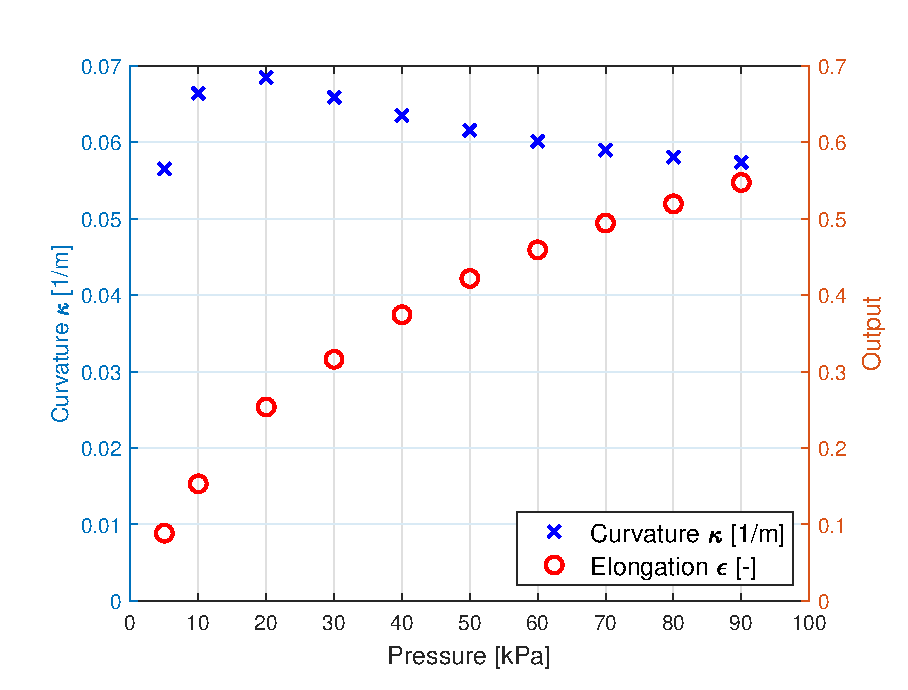
\includegraphics[width=\textwidth]{Figures/Chapter3/elongationvspressure.eps} 
        \caption{Elongation analysis, elongation and curvature as function of pressure.}
        \label{fig3:elongationvspressure}
    \end{minipage}\hfill
    \begin{minipage}{0.5\textwidth}
        \centering
        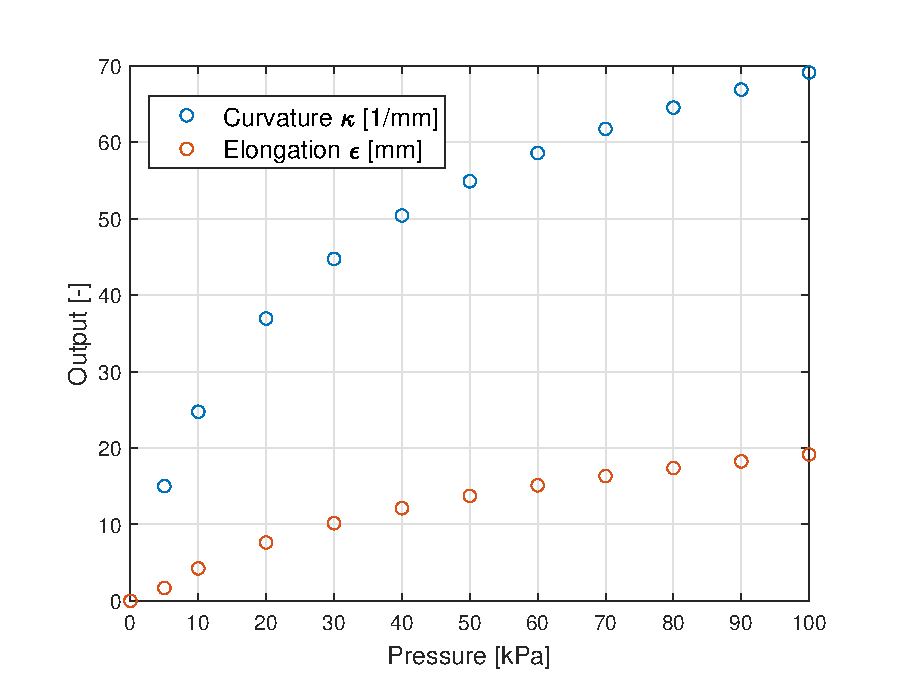
\includegraphics[width=\textwidth]{Figures/Chapter3/rotationvspressure.eps} 
        \caption{Curvature analysis, elongation and curvature as function of pressure.}
        \label{fig3:rotationvspressure}
    \end{minipage}
\end{figure}


\subsection{Curvature analysis}

\add{The curvature analysis allows to determine rotation stiffness of the robot manipulator. For this analysis only a single bellow is pressurized, while the other bellow pressure is kept zero. The pressurized bellow will result in a force. This force induces a moment around the center of the actuator, causing the actuator to curve. This results in a curvature as well as an elongation of the backbone curve. The result of this analysis is shown in Figure \ref{fig3:elongationvspressure}. It can be seen that the curvature and elongation rates decrease as pressure increases. From this experiment the rotation stiffness can be determined when the input mapping is known.}  


\section{Kinematic Model Fit}
\label{sec3:KinematicModelFit}

\add{The acquired data from the FEA is post-processed in Matlab to estimate the elongation and curvature of the analysis. This is done with the aid of the developed kinematic model. The kinematic model will be fitted through the nodal output of the FEA. The user can define the amount of shape functions used to approximate the shape of simulations. Increasing the amount of shape-functions will result in more flexibility. Therefore it can describe the actual deformation pattern better. However, fairly accurate approximations can be obtained when using a single-shape function. This means that each free strain, e.g. elongation and curvature, is described with a shape function polynomial of degree 1. Implying that the modal coordinates can be expressed as in Equation (\ref{eq3:q}). Expressing the curvature of the manipulator
} $\kappa \in \mathbb{R}$ \add{. and elongation} $\epsilon \in \mathbb{R}$. \add{ This means that the simulation results are approximated using the constant curvature approach.}\todo{explain constant curvature or cite a source.}

\begin{equation}
    q =  \begin{bmatrix} q_1 \\ q_2 \end{bmatrix}     = \begin{bmatrix} q_\kappa \\ q_\epsilon \end{bmatrix} 
    \label{eq3:q}
\end{equation}




\begin{figure}[H] 
  \begin{minipage}[b]{0.5\linewidth}
    \centering
    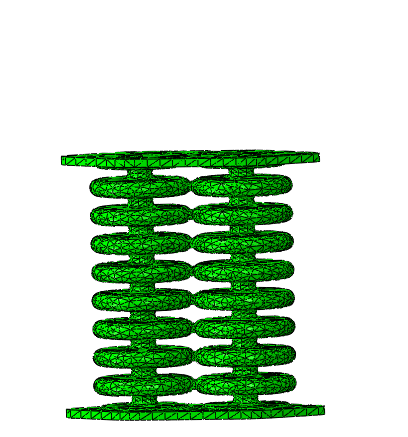
\includegraphics[width=\linewidth]{Figures/Chapter2/undeformed.png} 
    \caption{Undeformed FEA.} 
    \vspace{4ex}
    \label{fig3:FEMun} 
  \end{minipage}%%
  \begin{minipage}[b]{0.5\linewidth}
    \centering
    \includegraphics[width=\linewidth]{Figures/Chapter2/deformed60kpa.png} 
    \caption{Deformed FEA.} 
    \vspace{4ex}
    \label{fig3:FEMdef} 
  \end{minipage} 
  \begin{minipage}[b]{0.5\linewidth}
    \centering
    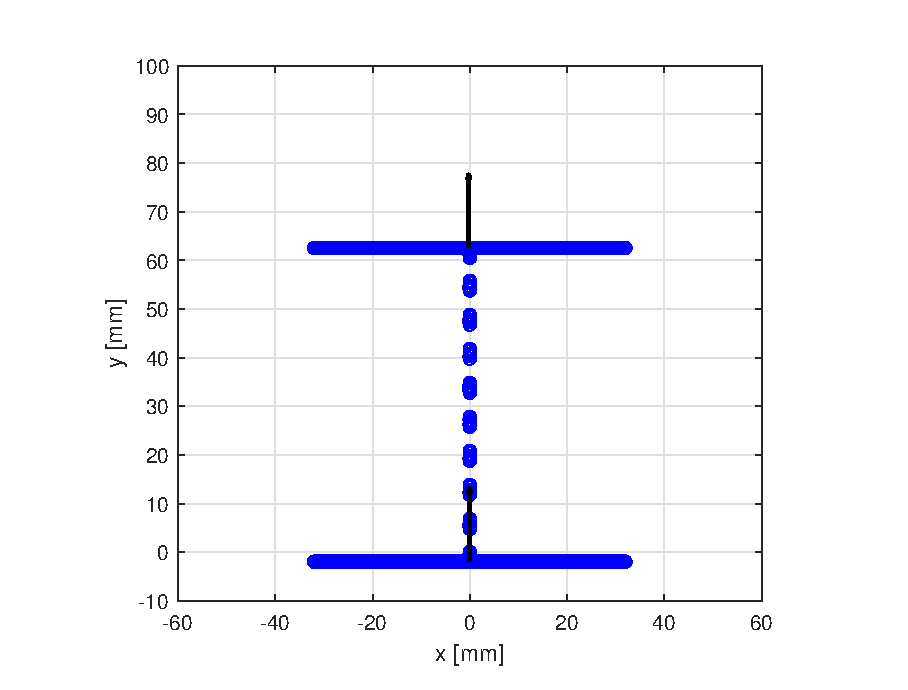
\includegraphics[width=\linewidth]{Figures/Chapter2/undeformednodal.eps} 
    \caption{Nodal image undeformed} 
    \vspace{4ex}
    \label{fig3:MATun} 
  \end{minipage}%% 
  \begin{minipage}[b]{0.5\linewidth}
    \centering
    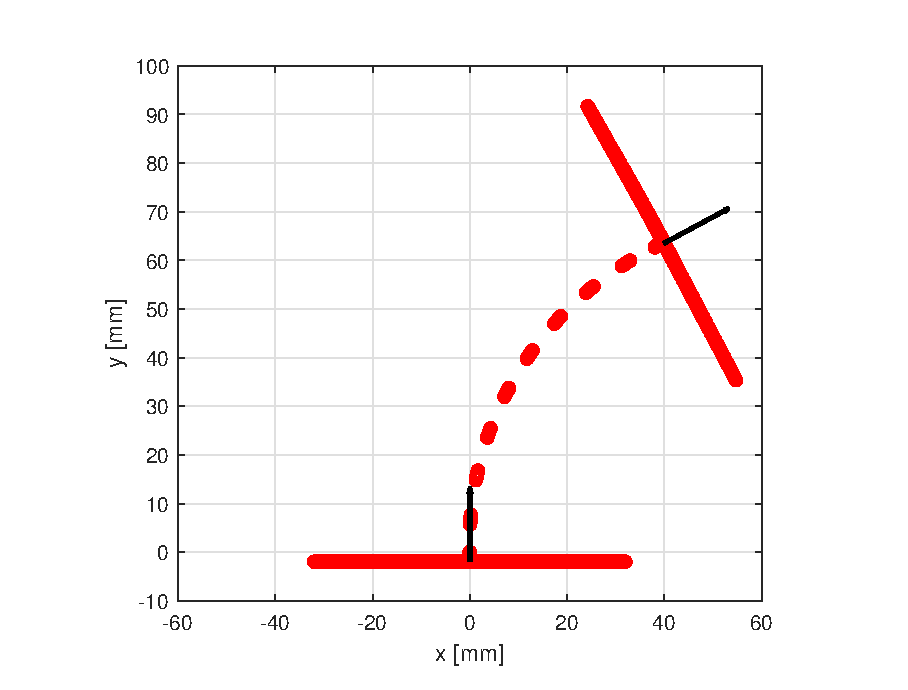
\includegraphics[width=\linewidth]{Figures/Chapter2/deformednodal.eps} 
    \caption{Nodal image deformed } 
    \vspace{4ex}
    \label{fig3:MATdef} 
  \end{minipage} 
\end{figure}
\todo{in this figure add crosses at the center cluster of nodes representing the backbone curve}

\add{Figures (\ref{fig3:FEMun}) and (\ref{fig3:FEMdef}) show the undeformed and deformed robotic manipulator in the finite element software, respectively. Their post-processed nodal image is shown in  Figures (\ref{fig3:FEMun}) and (\ref{fig3:FEMdef}), respectively. These images represent a curvature analysis where the left bellow is pressurized to 60 kPa. The nodal image shows clusters of nodes. The top and bottom plates, and backbone curve can clearly be distinguished. For the small clusters of nodes representing the backbone curve, the mass middle point has been determined. Denoted as vector } $\Bar{x}_{mid} \in \mathbb{R}^{2\times n}$ \add{containing the coordinates of each mass middle point. The approximate length of the backbone curve can be determined by using the function} \verb+arc_length.m+ \cite{arclength} \add{. This functions uses vector} $\Bar{x}_{mid}$ \add{ to approximate the arc length of this collection of coordinates. This estimated arc length is represented as } $\Bar{x}_{length} \in \mathbb{R}^+ $\add{is Matlab function }\verb+affine_fit.m+ \cite{affinefit} \add{is used to determine the orientation of the plane, hence the displayed normal vectors. Additionally, this function determines the mass middle point of the cluster of nodes representing the top plate. This point will be denoted as } $\Bar{x}_{end} \in \mathbb{R}^{2\times 1}$ \add{representing the coordinate of the end-effector.}

\add{An inverse kinematic configuration can fitted through the nodal displacement data. This is done via optimization with} \verb+fmincon.m+ \add{ To this end, the actuator is scaled to have length 1. This can be done by dividing all coordinates by the actuator length. The minimization problem that follows is}


\begin{equation}
\begin{aligned}
\min_{q} \hspace{5pt}  q^\top Q q  + \sum_{i=1}^{N}[\Phi_1(\Bar{x}_{mid} - f(q))^2] +   \Phi_2(\Bar{x}_{end}  - f(q)_{end})^2 +  \Phi_3(\Bar{x}_{length} - & f(q)_{length})^2  \\ 
\text{s.t.} \hspace{5pt} q_2 - 1 > 0
\end{aligned}
\end{equation}


\add{where} $Q \in \mathbb{R}^{n\times n}$ \add{is a diagonal weighing matrix used to penalize the value of the modal coordinates. This matrix} $Q$ \add{ is tuned to penalize high values of} $q$. \add{ Additional weighing factors} $\Phi_i \in \mathbb{R}^+$ and $i \in \{1,2,3\}$ \add{are applied to penalize individual terms. The used weights are, }

\begin{equation}
    Q = \begin{bmatrix}  0.01 & 0 \\ 0 & 0.01 \end{bmatrix} \hspace{25pt} \Phi_1 = 50  \hspace{25pt} \Phi_2 = 35 \hspace{25pt} \Phi_3 = 10
    \label{eq3:weights}
\end{equation}

\add{The only imposed constrained affects the elongation of the manipulator. Physically this constraint implies that the actuator can shorten in length, but the length can not become negative.}

\add{Figure (\ref{fig3:nodalfitelong}) and (\ref{fig3:nodalfitcurv}) show the result of fitting the inverse kinematic model through a set of nodal data. Figure (\ref{fig3:nodalfitelong}) shows a elongation analysis were both bellows are pressurized to 60 kPa. The modal coordinates belonging to this fit are } $q = [0.0036, 0.4472]^\top$. \add{The obtained modal coordinate expressing curvature again stresses the small curvature introduced with this analysis. Figure (\ref{fig3:nodalfitcurv}) shows a curvature analysis were the left bellow is pressurized to 60 kPa. The modal coordinates belonging to this fit are } $q = [0.91,0.24]^\top$.


\begin{figure}[H]
    \centering
\begin{minipage}{0.5\textwidth}
        \centering
        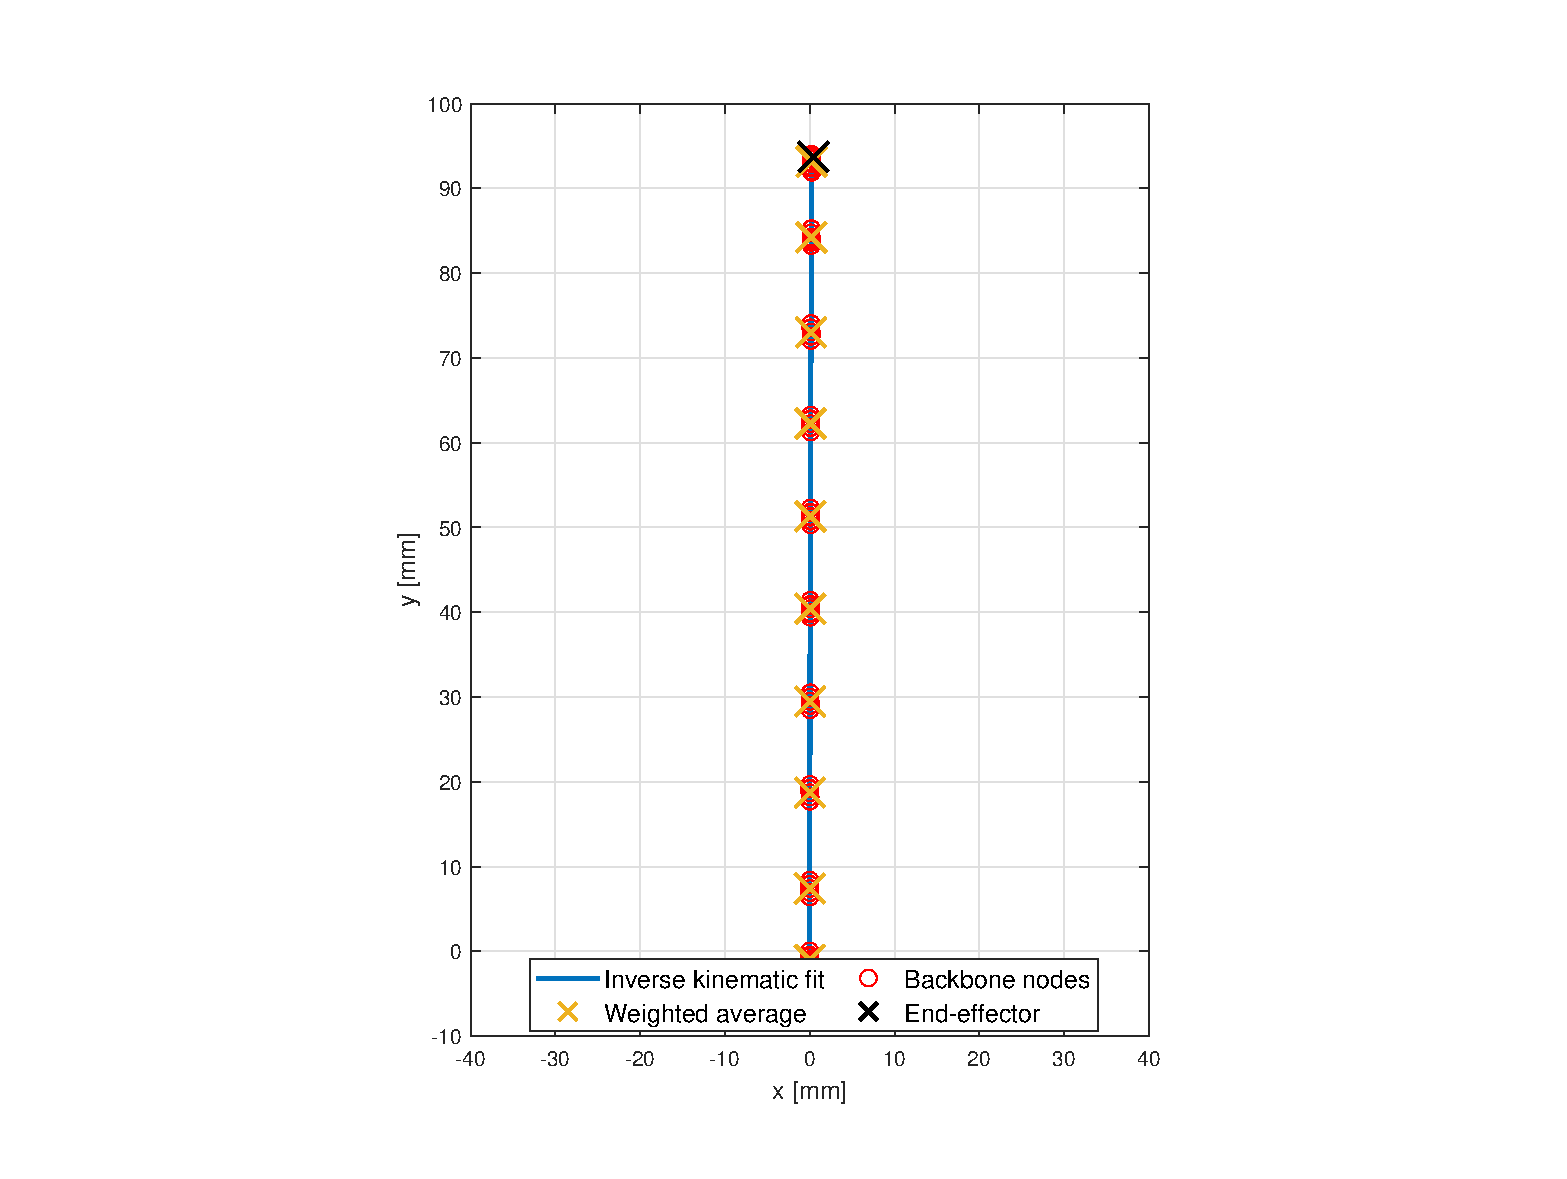
\includegraphics[width=\textwidth]{Figures/Chapter3/nodalfitelong.eps}
        \caption{Inverse kinematic fit for an elongation analysis. Both bellows pressurized to 60kPa.}
        \label{fig3:nodalfitelong}
    \end{minipage}\hfill
    \begin{minipage}{0.5\textwidth}
        \centering
        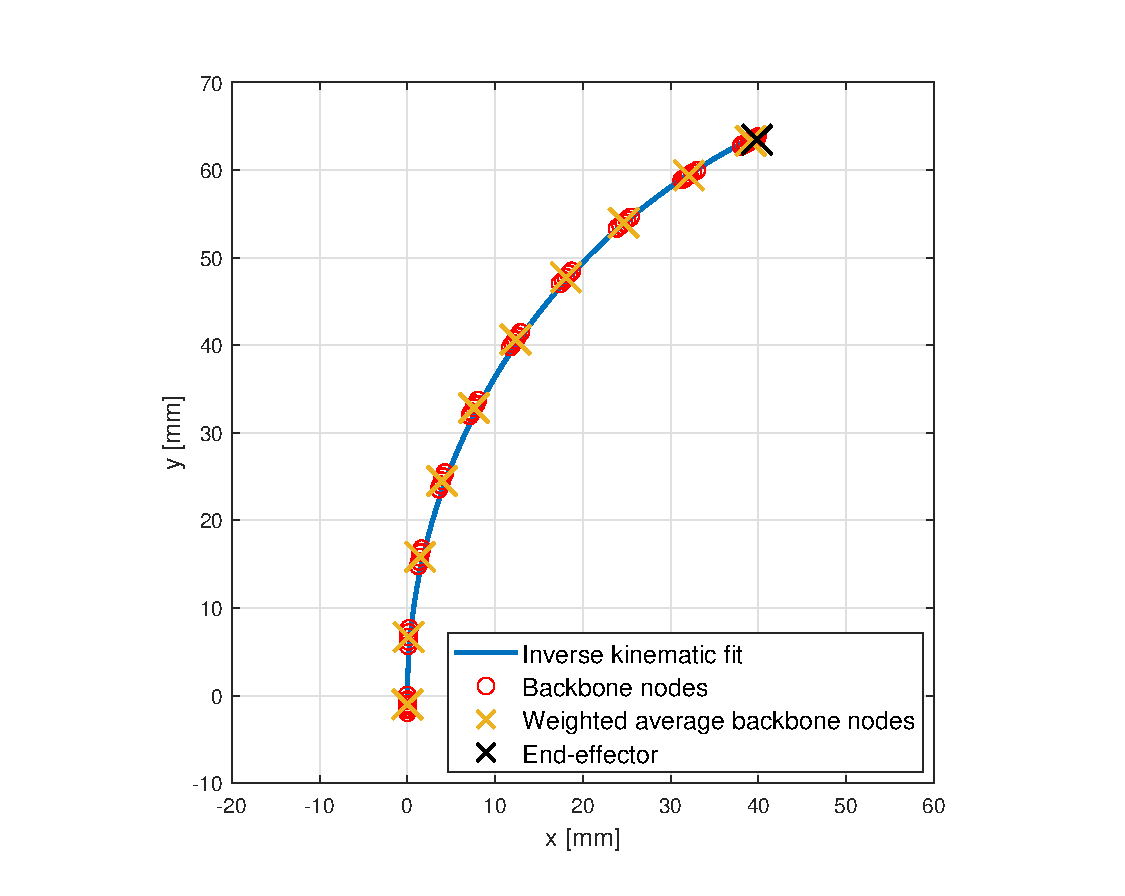
\includegraphics[width=\textwidth]{Figures/Chapter3/nodalfit.eps} 
        \caption{Inverse kinematic fit for a curvature analysis. Left bellow pressurized to 60kPa.}
        \label{fig3:nodalfitcurv}
    \end{minipage}
\end{figure}







\section{Input mapping}
\label{sec3:InputMapping}

\add{Stiffness is the ratio between applied force and elongation. To determine  stiffness for elongation and curvature, applied forces and direction of deformation is necessary. For the physical set-up, individual bellow pressure} $p_i \in \mathbb{R}^{\geq 0}$ with $i$ $\mathbb{N} \in \{1,2\}$ can be regulated. However, the control input in the dynamic model is force $F \in \mathbb{R}$ and moment $M \in \mathbb{R}$. Therefore, $H \in \mathbb{R}^{2 \times 2}$ is necessary to perform mapping $p \mapsto F$ and $p \mapsto M$ as,

\begin{equation}
     \begin{bmatrix} F \\ M \end{bmatrix}     = \underbrace{\begin{bmatrix}  a_1 & a_2 \\ a_3 & a_4 \end{bmatrix}}_{H}         \begin{bmatrix}  p_1 \\ p_2 \end{bmatrix}, \label{eq3:H}
\end{equation}

where entries of $H$ \add{are to be determined. Our aim is to decouple rotation and elongation. Therefore, it is important to understand that} $F$ \add{ causes elongation of the soft robotic actuator. Whereas, }$M$ \add{results in a curvature of the actuator. Therefore, the entries of }$a_1$ and $a_2$ \add{represent an effective surface area on which the pressure acts. Constant }$a_3$ and $a_4$ \add{represent a combination of effective surface area and lever on which the force acts. Due to symmetry properties it must hold that} $a_1 = a_2$ and $a_3 = -a_4$.

\add{First, the relation between pressure and force tried to be obtained. To this end, parameters} $a_1$ and $a_2$\add{ need to be determined. Finite element software} \verb+Abaqus/CAE+ \add{enables to study deformation of the soft actuator when applying pressure and forces. To map the pressure to force, multiple simulations will have to be carried out. First, elongation is determined for various bellow pressures. This is done by pressurizing both bellows equally for pressures between 0 and 100 kPa. This simulations will result in an elongation of the planar robot. Almost no rotation in observed, as the pressure in both bellows is equal.}




Additionally, out-of-plane displacement is hardly observed since the body is symmetric, and pressure acts perpendicular to this motion. Therefore, the pressurized bellows can be replaced by a pressure acting on the top of the actuator. This is done by constraining the top in lateral and transverse direction, only allowing elongation. This assumption is deemed valid since rotation and out-of-plane motion are negligible. Since the area of the top plate is known. The exact force applied to the top can be determined. Applying various pressures to the top plate and calculating elongation allows to obtain a relation between pressure and force.

Figure% (\ref{fig3:forcemapping}) shows the simulations marked with an 





\section{Stiffness results}



Assuming a hyper-elastic stiffness model \cite{Caasenbrood2020StiffnessModel}, the stiffness as function of elongation can be formulated as,


\begin{equation}
    k(\epsilon) =  \alpha_1 + \alpha_2 [\tanh({\alpha_3 \epsilon})^2 -1]
\end{equation}

The model has been fitted using $\verb+fmincon.m+$, where the following constrained is imposed
 $\alpha_1$  $>$ $\alpha_2$ $>$ 0. This results in $\alpha$ = $[33908,	335188,	-4.928]$







\begin{equation}
 \add{   K_\epsilon(q_1,q_2) = (1+0.88q_1)(\alpha_1 + \alpha_2\left[\tanh^2{(\alpha_3 q_2)}-1\right]) }
\end{equation}


\begin{equation}
 \add{   K_\kappa(q_1) = (\beta_1 + \beta_2\left[\tanh^2{(\beta_3 q_1)}-1\right]) }
\end{equation}


\begin{table}[H]
    \centering
\begin{tabular}{|c|c|c|c|} \hline
            &  $i = $ 1      &    $i = $    2   &  $i = $ 3  \\ \hline
   $\alpha_i$    &    1.1579e+3    & 1.1423e+3    & 3.134e-1 \\ \hline
   $\beta_i$     &  2.3008e+3    & 2.3008e+3    & 7.4204e-3 \\ \hline
\end{tabular}
    \caption{Parameters hyper-stiffness model}
    \label{tab:my_label}
\end{table}



